\subsection{Misure e osservazioni preliminari}

\paragraph{Punto di lavoro del PMT2}
Vogliamo trovare un buon punto di lavoro per il PMT2 che è alimentato con tensioni positive fino a $\sim \SI{800}{V}$. 
Mandiamo il segnale preamplificato del PMT2 all'amplificatore e la sua uscita all'ADC in modalità automatica.
Scegliamo di alimentare il PMT2 alla tensione consigliata di \SI{650}V. A questa tensione (e con guadagno dell'amplificatore impostato a $\times 1$) il fotopicco generato dai fotoni più energetici tra le sorgenti a disposizione (ovvero il picco a \SI{1.33}{MeV} del \co) si trova a $2/3$ della scala. Questo permette, agendo sul fattore di amplificazione del formatore/amplificatore di portare il fotopicco a fondo scala  e massimizzare la risoluzione dello spettrometro, mantenendo allo stesso tempo flessibilità nel caso la risposta del rivelatore non si rivelasse stabile\footnote{Cosa che abbiamo verificato essere vera: la posizione dei fotopicci può variare nel tempo fino al $\sim 10\%$.}.

\paragraph{Stabilità della risposta del PMT2}
Osservando l'istogramma dei campionamenti e notiamo che la risposta dello spettrometro è molto sensibile alle variazioni della tensione di alimentazione: da \SI{600}V a \SI{575}V, il valore in uscita si dimezza.
Il manuale dell'alimentatore riporta una stabilità dello $0.5\permil$ su \SI{24}h e dell' $1\permil$ su un mese. Volendo fare una stima otteniamo variazioni del $2/25 \times 600/1000 = 5\%$ in un mese, la metà in \SI{24}h. Sembra quindi che la stabilità della risposta del nostro spettrometro sia un limite importante nella nostra misura per cui nel seguito analizzeremo approfonditamente questo parametro.
%%%%%%%%%%%%%%%%%%%%%%%%%%%%%%%%%%%%%%%%%%%%%%%%%%%%%%%%%%%

\paragraph{Interazione con il bersaglio}
Poniamo lo scintillatore plastico (PMT1) davanti alla sorgente in modo che i raggi $\gamma$ possano interagire e subire scattering Compton. Osserviamo l'istogramma dei campionamenti del nostro spettrometro a vari angoli rispetto al bersaglio mentre l'ADC campiona in modalità automatica. 
Come è possibile vedere dalla \autoref{4ang} a piccolo angolo, quando lo spettrometro è direttamente attraversato dai fotoni che non interagiscono con il bersaglio, lo spettro è praticamente indistinguibile da quello acquisito senza bersaglio. A grandi angoli dovremmo vedere i fotoni che hanno fatto scattering Compton sul bersaglio e che dovrebbero riprodurre un circa lo stesso spettro ma traslato a energie minori, tuttavia come è chiaro dalla  \autoref{4ang} i fotoni che interagiscono sul muro subito dietro lo spettrometro o sul ferro (?CIPPALIPPA) del collimatore sovrastano in statistica il segnale che vorremmo osservare.\marginpar{Ci mettiamo una breve spiegazione della forma degli spettri o fottesega? (Bob)}

\begin{figure}[h]
\centering

\subfloat
{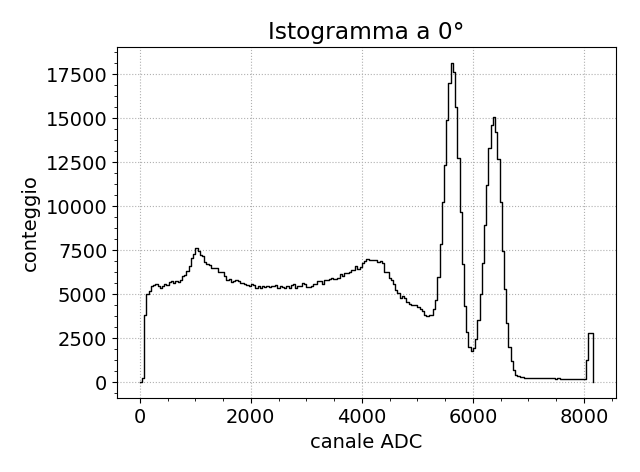
\includegraphics[width= 16 em]{0g}} \qquad
\subfloat
{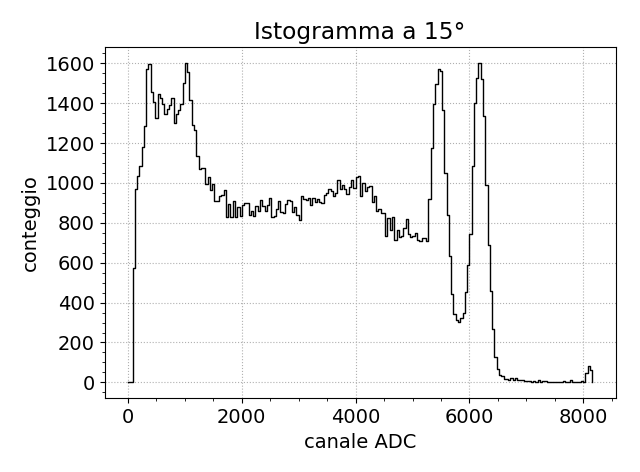
\includegraphics[width= 16 em]{15g}} \\

\subfloat
{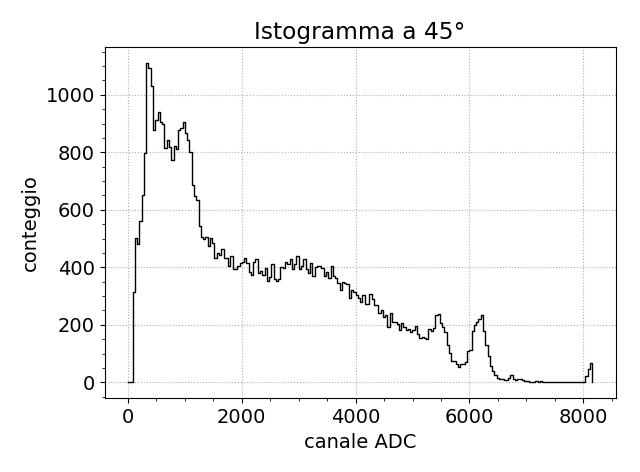
\includegraphics[width= 16 em]{45g}} \qquad
\subfloat
{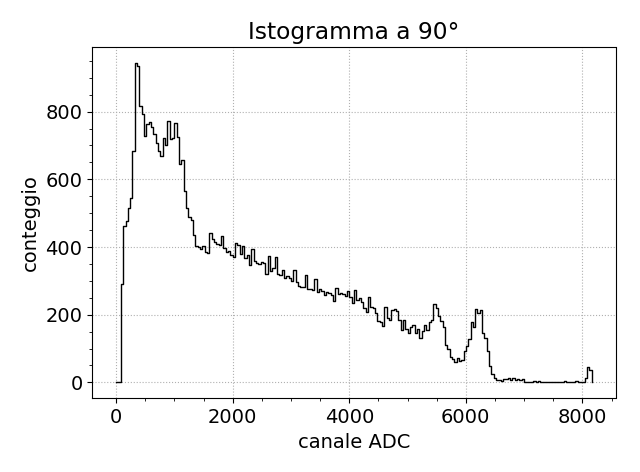
\includegraphics[width= 16 em]{90g}}

\caption{Spettri raccolti (in modalità automatica) a diversi angoli rispetto al bersaglio.}
\label{4ang}
\end{figure}

\marginpar{La parte che segue è abbastanza inutile se non aggiungiamo la spiegazione che dicevo prima (Bob)}
Abbiamo poi confrontato lo spettro a \SI{45}{\degree} con o senza scintillatore plastico, ma non abbiamo notato nessuna differenza. Abbiamo anche verificato che, come atteso, il rate di eventi diminuisce all'aumentare della distanza.
\marginpar{forse alcune di queste considerazioni sono stupide, ma è più facile togliere che aggiungere}

L'ultima acquisizione di questa serie è diversa rispetto alle altre: lo scintillatore cristallino è stato schermato lateralmente e superiormente per ridurre il backscattering. L'istogramma di \autoref{casetta} mostra come questo fenomeno sia evidentemente diventato più raro.

\begin{figure}
\centering
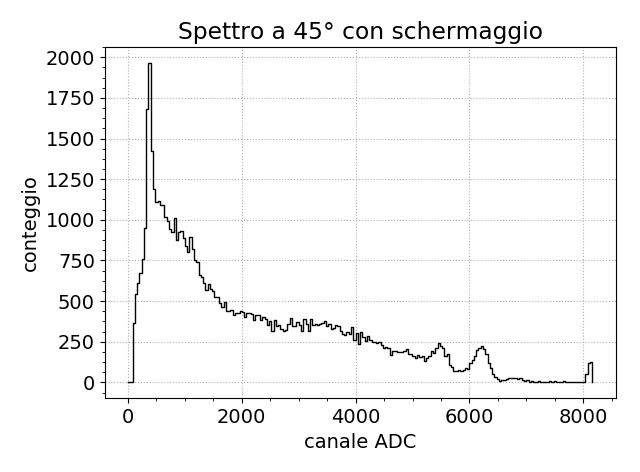
\includegraphics[width=25 em]{45gs}
\caption{Spettro energetico del PMT2 con schermaggio superiore e laterale.}
\label{casetta}
\end{figure}

\paragraph{Trigger esterno} Prima di esporre i risultati ottenuti illustriamo il funzionamento del circuito adoperato.\\
Vogliamo acquisire i segnali ogni volta che l'uscita negativa di breve durata (qualche \si{ns}) del PMT2 supera una certa soglia. L'ampiezza tipica di questo segnale vale \SI{20}{mV}, perciò deve essere amplificata per poter essere letta dal discriminatore a nostra disposizione che ha una soglia minima di \SI{35}{mV}. Colleghiamo allora questa uscita ad una amplificatore 10x 
\marginpar{spero che gradiscano la notazione ``10x'' \\  ci vuole anche il disegno}
e mandiamo poi il segnale al solito discriminatore con soglia al minimo.

Per registrare il segnale dobbiamo provvedere alla costruzione di un trigger per l'ADC che, come specificato dalla documentazione, deve partire almeno \SI{200}{ns} prima del picco e deve terminare almeno \SI{200}{ns} dopo. Usando l'oscilloscopio, ritardiamo il segnale del discriminatore e lo allunghiamo attraverso l'uso di un modulo \texttt{gate \& delay} non retriggerabile. Scegliamo di farlo durare \SI{550}{ns} prima e dopo il picco del formatore.

Colleghiamo il cavo coassiale che trasmette l'uscita del formatore all'ingresso ``gate'' dell'ADC facendo un parallelo con un tappino da \SI{50}{\Omega} perché questo ingresso ha una impedenza alta e il nostro accorgimento evita la deformazione del segnale.
Modifichiamo il file di configurazione in modo che l'ADC acquisisca soltanto quando il trigger è attivo. Notiamo che la soglia appena utilizzata elimina tutti i segnali inferiori ai 1000 digit. 
